% ****** Start of file apssamp.tex ******
%
%   This file is part of the APS files in the REVTeX 4.1 distribution.
%   Version 4.1r of REVTeX, August 2010
%
%   Copyright (c) 2009, 2010 The American Physical Society.
%
%   See the REVTeX 4 README file for restrictions and more information.
%
% TeX'ing this file requires that you have AMS-LaTeX 2.0 installed
% as well as the rest of the prerequisites for REVTeX 4.1
%
% See the REVTeX 4 README file
% It also requires running BibTeX. The commands are as follows:
%
%  1)  latex apssamp.tex
%  2)  bibtex apssamp
%  3)  latex apssamp.tex
%  4)  latex apssamp.tex
%
\documentclass[%
 reprint,
nofootinbib,
%superscriptaddress,
%groupedaddress,
%unsortedaddress,
%runinaddress,
%frontmatterverbose,
%preprint,
%showpacs,preprintnumbers,
%nofootinbib,
%nobibnotes,
%bibnotes,
aps,
%pra,
%prb,
%rmp,
%prstab,
%prstper,
%floatfix,
]{revtex4-1}

\usepackage[utf8]{inputenc}
\usepackage[english]{babel}
\usepackage{dsfont}
\usepackage{amsmath}
\usepackage{ mathrsfs }
\usepackage{amssymb}
\usepackage{graphicx}% Include figure files
\usepackage{dcolumn}% Align table columns on decimal point
\usepackage{bm}% bold math
\usepackage{amsmath}
\usepackage{varioref}
\usepackage{booktabs}
\usepackage[bottom]{footmisc}

\usepackage{algpseudocode}
\usepackage{listings}

\usepackage{lmodern}
\usepackage{tikz}
\usepackage{kantlipsum}
\usetikzlibrary{calc,patterns,angles,quotes}

\newcommand{\RN}[1]{%
  \textup{\uppercase\expandafter{\romannumeral#1}}%
}


\newcolumntype{C}{>{$}c<{$}}
\AtBeginDocument{
\heavyrulewidth=.08em
\lightrulewidth=.05em
\cmidrulewidth=.03em
\belowrulesep=.65ex
\belowbottomsep=0pt
\aboverulesep=.4ex
\abovetopsep=0pt
\cmidrulesep=\doublerulesep
\cmidrulekern=.5em
\defaultaddspace=.5em
}

%\usepackage{hyperref}% add hypertext capabilities
%\usepackage[mathlines]{lineno}% Enable numbering of text and display math
%\linenumbers\relax % Commence numbering lines

%\usepackage[showframe,%Uncomment any one of the following lines to test
%%scale=0.7, marginratio={1:1, 2:3}, ignoreall,% default settings
%%text={7in,10in},centering,
%%margin=1.5in,
%%total={6.5in,8.75in}, top=1.2in, left=0.9in, includefoot,
%%height=10in,a5paper,hmargin={3cm,0.8in},
%]{geometry}

\begin{document}

%\preprint{APS/123-QED}

\title{The Solar System}% Force line breaks with \\


\author{Ivar Svalheim Haugerud}\homepage{http://www.github.uio.no/ivarsh/FYS4150}
\author{Cecilie Glittum}\homepage{http://www.github.uio.no/cecilgl/FYS4150}

\affiliation{%
 Department of Physics, University of Oslo\\
}%


\date{\today}% It is always \today, today,
             %  but any date may be explicitly specified

\begin{abstract}
By solving coupled differential equations numerically, through discretizing and using natural units, for the Solar System, we are able to reproduce analytical results and compare the velocity Verlet and forward Euler algorithm.
We study the two body problem to test the precision of our algorithm, finding that the velocity Verlet algorithm produce a more precise results, as well as conserving angular momentum and energy to an accuracy good enough for all practical purposes. Velocity Verlet is therefore superior to the forward Euler algorithm, even though it requires approximately a factor of two more FLOPS. The system is expanded to a three body problem in order to test our assumption that the center of mass is fixed at the center of the Sun. We find that this assumption changes the position of planet's by around $0.008$AU. Using the bisection method we are able to find the escape velocity of the Earth. Analytically the escape velocity is $8.8857$AU/year, numerically we find it to be $8.8851(5)$AU/year. We study the effects of altering the exponent of Newton's gravitational law, and find that the orbit of Earth gradually becomes more unstable as the exponent approaches $3$, and diverges when the exponent is equal to $3$. By Taylor approximation we add a relativistic term from Einstein's general theory of relativity to Newton's gravitational law. We find that with this additional term we are able to reproduce the analytical value of Mercury's perihelion precision, $42.98^{''}$ per century, numerically with $42.91(1)^{''}$ per century, which is a relative deviation of $0.17\%$.
\end{abstract}
\maketitle


\section{Introduction}
Understanding the movement of celestial objects in our Solar System was one of the major triumph's during the birth of physics. Isaac Newton developed his gravitational law to explain why the moon orbits the Earth, and why the Earth orbit the Sun etc. The orbits were then possible to calculate using differential calculus, which Newton also was a major contributor to the development off. The systems we can solve with pen and paper is heavily limited, where the two-body problem is largest number of objects we can find a general solution for. With the development of computers we can find very close to exact solution to many body problems.\par Many-body problems are often described by a set of coupled differential equations as an initial value problem. There exists a large variety of algorithms for solving such equations. Since we study a physical system, we're interested in methods which conserve the total energy and angular momentum precisely. This is something we study in this article, where we compare the conservation properties for the forward Euler algorithm and the velocity Verlet algorithm. As well as finding how well they produce correct positions. These results will be compared to the number of FLOPS and computational time used by both algorithms. The physical system we test these algorithms on is the Solar System.\\

When studying the Solar System, we have included data from NASAs JPL HORIZONS\footnote{Go to \url{http://ssd.jpl.nasa.gov/horizons.cgi#top} and change from OBSERVER to VECTOR.} for the initial positions and velocities of the objects used in the calculations. The data was collected 2018-Sep-28 00:00:00.0000 TDB. With these values we will be able to produce the exact positions and velocities of all objects in our Solar system in three dimensions for the coming years.

To solve the coupled differential problem for $N$ bodies in three dimensions we implement the solver through object orientation. This gives us the ability to run the same, general code, for many different cases of our solar system. Thus we can easily start by verifying the implementation of our algorithms by looking at the a special case of the system with an analytical solutions, the two body problem. If the results fit the theory we can easily add more objects to the solver, and guarantee correct results. In addition we are able to make sub-classes which inherits variables and functions from their mother-class. This way we can write the code once, and use it many times. Using this class we are able to test different results of celestial mechanics. We will find the escape velocity of the Earth, and the change of the Earth's orbit if Newton's gravitational law was different. In addition we will check one of the most important tests of Albert Einstein's general theory of relativity, the perihelion precision of Mercury.

In this article we will start by going through the theory used, how the algorithm incorporates them, and how we use these algorithms to answer the questions we are interested in. We go through the results we produce, and discuss the results and their implications, before concluding on our work.

\section{Theory}

\subsection{The differential equations}
The trajectory of the objects in the Solar System is governed by Newton's gravitational law, which states that the force acting between two objects is
\begin{equation}
\vec{F}_{ij} = G\frac{M_i M_j}{r^3}\vec{r}, \label{newton}
\end{equation}
where $G$ is the gravitational constant, $M_i$ and $M_j$ are the masses of the considered objects and $r$ is the distance between them. It is important that the force-vector points away from the object the force is acting on, thus if this is the force of object $j$ on object $i$, $\vec{r} = \vec{r}_j - \vec{r}_i$, where $\vec{r}_i$ is the position vector of object $i$. When using this law we let the force act on the center of mass of the objects, and indirectly approximate them as point particles.

The total force acting on an object in the Solar System is thus given as
\begin{equation}
\vec{F}_i = \sum_{j \neq i} \vec{F}_{ij}.
\end{equation}
By Newton's second law, we get a relation between the acceleration of an object and the force acting on it.
\begin{equation}
\vec{a}_i = \frac{\vec{F}_i}{m}
\end{equation}
We see that since the forces $\vec{F}_i$ depends on the positions of all the objects in the system, the accelerations are also dependent on the positions of all objects in the system. The relations between acceleration, velocity and position is given by the following differential equations
\begin{align}
  \begin{split}
\frac{d\vec{v}}{dt} &= \vec{a},\\
\frac{d\vec{\vec{r}}}{dt} &= \vec{v}. \label{coupled_diff}
  \end{split}
\end{align}
Knowing the position of all objects in our system we can calculate the force acting on each body, and from this solve a set of coupled differential equations to find their position over time.

\subsection{Escape velocity}
The escape velocity of the Earth can be found by setting the total energy of the Earth to be greater than zero, such that it is not in a bounded state. When considering the Sun-Earth system, we have that
\begin{equation}
E_{Earth} = \frac{1}{2}M_{Earth}v^2 -G\frac{M_\odot M_{Earth}}{r^2}.
\end{equation}
If we constrain this to be grater than zero and insert values for the quantities in units of AU, years and Sun masses, $G = 4\pi^2$, as we will show later, we have
\begin{align}
\frac{1}{2}M_{Earth}v^2 -G\frac{M_\odot M_{Earth}}{r^2} &> 0\\
v &> \sqrt{2G\frac{M_\odot }{r^2}}\\
v &> 2\pi\sqrt{2}.
\end{align}
For the Earth to escape the gravitational pull of the Sun, starting $1$AU away, it needs an initial velocity equal to $2\pi\sqrt{2}$AU/year.

\subsection{Constants of motion}\label{const_mot}


%We consider an $n$-body system with generalized coordinates $q \in \{r_1, r_2, \dots, r_n, \theta_1, \theta_2, \dots, \theta_n\}$. When writing out the full Lagrangian of the system, we get
%\begin{equation}
%L = \sum_{i}\frac{1}{2}m_i(\dot{r}_i + r^2_i\dot{\theta}_i) - \sum_{i}\sum_{j}\left(-\frac{1}{2}G\frac{m_im_j}{r_{ij}}\right)
%\end{equation}

The gravitational force is a conservative force, which follows from the fact that the force can be written as the negative gradient of a potential. For a system where we only have conservative forces, energy is conserved. This follows from the energy principle: ``The change in (mechanical) energy is equal to the work done by non-conservative forces"\cite{malthe}. Another constant of motion is the total angular momentum of the system, $\vec{L}$. The total angular momentum is conserved, as there are no external torque working on the system. Thus
\begin{equation}
\frac{d}{dt}\vec{L} = \tau_{\mathrm{ext}} = 0.
\end{equation}
Since we know that these quantities have to stay constant during the evolution of the system, we can test the quality of the algorithms by checking if they conserves energy and angular momentum.

\subsection{Generalization of Newton's gravitational law}\label{change_beta_section}

We want to study modifications of Newton's gravitational law on the form
\begin{equation}
\vec{F}_{ij} = G\frac{M_iM_j}{r_{ij}^\beta}\vec{e}_r. \label{newton_betta}
\end{equation}
When studying the Sun-Earth system, and approximating the Sun to be the center of mass, we have only one force acting, namely the gravitational force on the Earth from the Sun:
\begin{equation}\label{eq: beta_force}
\vec{F} = G\frac{M_\odot M_{Earth}}{r^\beta}\vec{e}_r,
\end{equation}
where $\vec{r}$ is the position vector of the Earth. By integrating we find that the corresponding potential is
\begin{equation}
V = \frac{1}{\beta - 1}\frac{GM_\odot M_{Earth}}{r^{\beta - 1}} = \frac{1}{\alpha}\frac{GM_\odot M_{Earth}}{r^{\alpha}},
\end{equation}
where $\alpha = \beta -1$.

\begin{figure}
\centering
    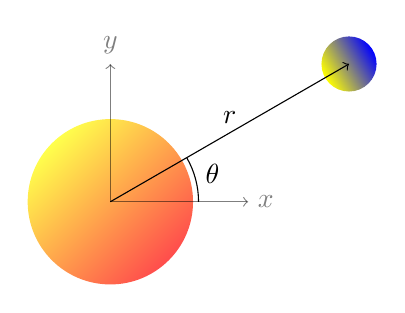
\begin{tikzpicture}[scale=3.5]
        \def\rS{0.3}                                % Sun radius

        \def\Earthangle{30}                         % angle wrt to horizontal
        \def\rE{0.1}                                % Earth radius
                                                    % Major radius of Earth's elliptical orbit = 1
        \def\eE{0}                               % Excentricity of Earth's elliptical orbit
        \pgfmathsetmacro\bE{sqrt(1-\eE*\eE)}        % Minor radius of Earth's elliptical orbit

        %\def\Moonangle{-45}                         % angle wrt to horizontal
        %\pgfmathsetmacro\rM{.7*\rE}                 % Moon radius
        %\pgfmathsetmacro\aM{2.5*\rE}                % Major radius of the Moon's elliptical orbit
        \def\eM{0.4}                                % Excentricity of Earth's elliptical orbit
        %\pgfmathsetmacro\bM{\aM*sqrt(1-\eM*\eM)}    % Minor radius of the Moon's elliptical orbit
        %\def\offsetM{30}                            % angle offset between the major axes of Earth's and the Moon's orbits



        % This function computes the direction in which light hits the Earth.
        \pgfmathdeclarefunction{f}{1}{%
            \pgfmathparse{
                ((-\eE+cos(#1))<0) * ( 180 + atan( \bE*sin(#1)/(-\eE+cos(#1)) ) )
                +
                ((-\eE+cos(#1))>=0) * ( atan( \bE*sin(#1)/(-\eE+cos(#1)) ) )
            }
        }

        % This function computes the distance between Earth and the Sun,
        % which is used to calculate the varying radiation intensity on Earth.
        \pgfmathdeclarefunction{d}{1}{%
            \pgfmathparse{ sqrt((-\eE+cos(#1))*(-\eE+cos(#1))+\bE*sin(#1)*\bE*sin(#1)) }
        }

        % Draw the elliptical path of the Earth.
        %\draw[thin,color=gray] (0,0) ellipse (1 and \bE);

        % Draw the Sun at the right-hand-side focus
        \shade[
            top color=yellow!70,
            bottom color=red!70,
            shading angle={45},
            ] ({sqrt(1-\bE*\bE)},0) circle (\rS);
         %\draw ({sqrt(1-\b*\b)},-\rS) node[below] {Sun};


        % Draw the Earth at \Earthangle
        \pgfmathsetmacro{\radiation}{100*(1-\eE)/(d(\Earthangle)*d(\Earthangle))}
        \colorlet{Earthlight}{yellow!\radiation!blue}
        \shade[%
            top color=Earthlight,%
            bottom color=blue,%
            shading angle={90+f(\Earthangle)},%
        ] ({cos(\Earthangle)},{\bE*sin(\Earthangle)}) circle (\rE);
        %\draw ({cos(\Earthangle)},{\bE*sin(\Earthangle)-\rE}) node[below] {Earth};

        % Draw the Moon's (circular) orbit and the Moon at \Moonangle
        %\draw[thin,color=gray,rotate around={{\offsetM}:({cos(\Earthangle)},{\bE*sin(\Earthangle)})}]
          %  ({cos(\Earthangle)},{\bE*sin(\Earthangle)}) ellipse ({\aM} and {\bM});
       % \shade[
          %  top color=black!70,
           % bottom color=black!30,
           % shading angle={45},
       % ]   ({cos(\Earthangle)+\aM*cos(\Moonangle)*cos(\offsetM)-\bM*sin(\Moonangle)*sin(\offsetM)},%
       %     {\bE*sin(\Earthangle)+\aM*cos(\Moonangle)*sin(\offsetM)+\bM*sin(\Moonangle)*cos(\offsetM)}) circle (\rM);


\coordinate (origo) at (0,0);
\coordinate (Earth) at ({cos(\Earthangle)},{\bE*sin(\Earthangle)});
\coordinate (x) at (0.5,0);

\draw [->] (0,0) -- ({cos(\Earthangle)},{\bE*sin(\Earthangle)});

\node at ({cos(\Earthangle)/2},{\bE*sin(\Earthangle)/2}) [above] {$r$};

\pic [draw, "$\theta$", angle eccentricity=1.2, angle radius = 1.12cm] {angle = x--origo--Earth};



\draw [->, opacity = 0.5] (0,0) -- (0.5,0);
\node at (0.5,0) [right, opacity = 0.5] {$x$};
\draw [->, opacity = 0.5] (0,0) -- (0,0.5);
\node at (0,0.5) [above, opacity = 0.5] {$y$};

    \end{tikzpicture}
    \caption{The Sun and Earth with the generalized coordinates $r$ and $\theta$. The Sun is assumed to be at rest at the origin.}\label{fig: Sun-Earth-fig}
\end{figure}

When studying this problem in two dimension, the Earth has two degrees of freedom, and the system can therefore be described by two generalized coordinates: $r$ and $\theta$, as shown in Fig. \ref{fig: Sun-Earth-fig}. The position vector of the Earth is then
\begin{equation}
\vec{r} = r(\cos\theta, \sin\theta).
\end{equation}
the Lagrangian, kinetic energy minus potential energy, of the system is
\begin{equation}
  \mathscr{L} = \frac{1}{2}M_{Earth}\left(\dot{r}^2 + r^2\dot{\theta}^2\right) - \left(-\frac{1}{\alpha}\frac{GM_\odot M_{Earth}}{r^\alpha}\right).
\end{equation}
In Appendix \ref{eom} we show that by using conservation of angular momentum, the Lagrangian can be reduced to a one dimensional Lagrangian
\begin{equation}
  \mathscr{L} = \frac{1}{2}M_{Earth}\dot{r}^2 - V_{\mathrm{eff}}(r),
\end{equation}
where we define the effective potential as
\begin{equation}\label{eq: effective_potential}
V_{\mathrm{eff}}(r) = \frac{1}{2}\frac{l^2}{M_{Earth}}\frac{1}{r^2} - \frac{1}{\beta - 1}\frac{GM_\odot M_{Earth}}{r^{\beta - 1}}.
\end{equation}
In Appendix \ref{eom} it is also shown that for this effective potential to have any stable equilibrium, we must have
\begin{equation}
\beta < 3.
\end{equation}
The stability of the orbit of the Earth will vary for different values of $\beta$, and for the orbit to be stable $\beta<3$.

\subsection{Relativistic corrections to Newton's gravitational law}\label{GR}

By doing a Taylor expansion of the field equations of Albert Einstein's general theory of relativity (GR) to first order in $1/c^2$, Newton's gravitational law gets an additional relativistic correction:
\begin{equation}
\vec{F}_{ij}= G\frac{M_i M_j}{r_{ij}^2}\left[ 1 + \frac{l_{ij}^2}{r_{ij}^2c^2} \right]. \label{GR_force}
\end{equation}
This extra term will give a contribution to the gravitational force which changes the position of the perihelion point of orbit over time. As the additional term is often negligible, the effect is small, but can still be observed for fast moving planets, with a short period. The contribution to the perihelion precision from GR is given by \cite{einstein}
\begin{equation}
\epsilon = 24\pi^3 \frac{a^2}{T^2c^2(1-e^2)},
\end{equation}
where $e$ is the orbital eccentricity, $a$ the semi-major axis, and $T$ the orbital period. The planet with the smallest orbital period is Mercury. When inserting values for all these quantities, one get that the perihelion precision of Mercury due to relativistic corrections is $42.97^{\prime\prime}$ per century.


\section{Algorithms}
In order to find the position of all bodies as time evolves we need to solve the set of coupled differential equations \eqref{coupled_diff} where we find the acceleration from Newton's gravitational force \eqref{newton}, for an arbitrary number of objects. For our system this set of coupled differential equations is only possible to solve numerically.

The first step in solving these equations numerically is to scale and discretize them. When working with the Solar System, the best units to use is AU for lengths, years for time, and Sun masses for masses. By looking at the Sun - Earth system, we can find a value for the gravitational constant in these new units. If we take the orbit of the Earth around the Sun to be circular, we have
\begin{equation}
F_{Earth} = M_{Earth}\frac{v^2}{r} = G \frac{M_{Earth} M_\odot}{r^2}.
\end{equation}
This gives
\begin{equation}
G M_\odot = v^2r = (2\pi \mathrm{AU/yr})^2 1\mathrm{AU} = 4\pi^2 \mathrm{AU^3/yr^2},
\end{equation}
thus, we will use
\begin{equation}
G =  4\pi^2 \mathrm{AU^3/(yr^2}M_\odot ).
\end{equation}

We discretize the equations as C. Glittum and I. Haugerud \citep{project1}. Instead of a boundary value problem we consider an initial value problem. By knowing the initial time $T_0$, and the final time, $T_{max}$, for the coupled differential equation, we get, by using the number of integration points, $N$, the following discretized $t$-values
\begin{equation}
t_i = T_0+hi,
\end{equation}
where $i = 0, 1, 2, ... , N-1$ and
\begin{equation}
h = \frac{T_{max}-T_0}{N-1}.
\end{equation}


We need a numerical algorithm for solving these coupled differential equations. In this article, we consider two different algorithms: Forward Euler (FE) and velocity Verlet (VV). Both these methods are based on Taylor expansions of functions
\begin{equation}\label{eq: Taylor}
f(x \pm h) = f(x) \pm h\frac{df}{dx}(x) + \frac{1}{2!}h^2\frac{d^2f}{dx^2}(x) + \dots.
\end{equation}
To derive these algorithms different combinations of the Taylor expansion of a general function can be added or subtracted from each other.

\subsection{Forward Euler}
The forward Euler algorithm uses the two first terms of the Taylor expansion to approximate the next step,
\begin{align}
\vec{x}_{i+1} &= \vec{x}_i + h \vec{v}_i,\\
\vec{v}_{i+1} &= \vec{v}_i + h \vec{a}_i.
\end{align}
When including all the steps, this algorithm can be written in pseudo code as
\begin{algorithmic}[H]
\State compute $h$
\State initialize $\vec{x}_0$ and $\vec{v}_0$
\For  {i = 0, 1, 2, ..., N-1}
	\State compute $\vec{a}_i$ from forces
	\State $\vec{x}_{i+1} = \vec{x}_i + h \vec{v}_i$
	\State $\vec{v}_{i+1} = \vec{v}_i + h \vec{a}_i$
\EndFor
\State
\end{algorithmic}
This calculation has $4N$ FLOPS, without considering the FLOPS from calculating the acceleration, but trades the efficiency with accuracy, and has a local error which goes as $\mathcal{O}(h^2)$ for both $\vec{x}$ and $\vec{v}$


\subsection{Velocity Verlet}

The velocity Verlet algorithm is known for being better when working with Hamiltonian systems, as it conserves energy more precisely. This algorithm uses the three first terms of the Taylor expansion, Eq. \eqref{eq: Taylor}, i.e. it includes one more term of the Taylor expansion compared to forward Euler:
\begin{align}
\vec{x}_{i+1} &= \vec{x}_i + h\vec{x}_i^{\prime} + \frac{h^2}{2!}\vec{x}_i^{\prime\prime} + \mathcal{O}(h^3),\\
\vec{v}_{i+1} &= \vec{v}_i + h\vec{v}_i^{\prime} + \frac{h^2}{2!}\vec{v}_i^{\prime\prime} + \mathcal{O}(h^3).
\end{align}
We know the values for $\vec{x}_i^{\prime} = \vec{v}_i$, $\vec{x}_i^{\prime\prime} = \vec{v}_i^{\prime} = \vec{a}_i$. On the other hand, the value of $\vec{v}_i^{\prime\prime}$ is unknown, and we need to approximate it.
By Taylor expansion of $\vec{v}_{i+1}^{\prime}$, we have
\begin{equation}
\vec{v}_{i+1}^{\prime} = \vec{v}_i^{\prime} + h\vec{v}_i^{\prime\prime} + \mathcal{O}(h^2).
\end{equation}
Thus
\begin{equation}
h\vec{v}_i^{\prime \prime} \approx \vec{v}^{\prime}_{i+1} - \vec{v}_i^{\prime} = \vec{a}_{i+1} - \vec{a}_i
\end{equation}
This leaves us with
\begin{align}
\vec{x}_{i+1} &= \vec{x}_i + h\vec{v}_i + \frac{h^2}{2}\vec{a}_i + \mathcal{O}(h^3),\\
\vec{v}_{i+1} &= \vec{v}_i + \frac{h}{2}\left( \vec{a}_{i+1} + \vec{a}_i \right) + \mathcal{O}(h^3).
\end{align}

The clue when actually implementing this algorithm is to calculate $\vec{a}_{i+1}$ between the calculation of $\vec{x}_{i+1}$ and the calculation of $\vec{v}_{i+1}$, as only $\vec{x}_{i+1}$ is needed for calculating $\vec{a}_{i+1}$, while $\vec{a}_{i+1}$ is needed for calculating $\vec{v}_{i+1}$.

The general algorithm using velocity Verlet is

\begin{algorithmic}[H]
\State compute $h$
\State initialize $\vec{x}_0$ and $\vec{v}_0$
\For  {i = 0, 1, 2, ..., N-1}
	\State compute $\vec{a}_i$ from forces
	\State $\vec{x}_{i+1} = \vec{x}_i + h\vec{v}_i + \frac{h^2}{2}\vec{a}_i$
	\State compute $\vec{a}_{i+1}$
	\State $\vec{v}_{i+1} = \vec{v}_i + \frac{h}{2}\left( \vec{a}_{i+1} + \vec{a}_i \right)$
\EndFor
\State
\end{algorithmic}
Where we achieve more accurate results compared to FE, and conserve energy more precisely, but pay the price by having $9N$ FLOPS in addition to having to calculate the forces twice for each $N$.

\section{Method}
\subsection{Sun at rest}
For testing our algorithm we want to study simple systems. We therefore start by looking at systems where we fix the position of the Sun at the origin. When forcing the Sun to stand still we are approximating the center of mass of the system to be equal to the center of mass of the Sun. We will discuss the validity of this assumption later.\\
Since our initial conditions are from NASA, the initial position of the Sun is not at the origin. Due to this we parallel shift all of the objects in our system, so that the Sun is at the origin, and all other objects are shifted accordingly.\\
If we keep the Sun at rest with only one object orbiting it, we can achieve perfectly circular orbits. We do this for the Sun-Earth system. This will be used to test the precision of our algorithm. With the correct initial velocity we will know where the position of the Earth will be after one year, exactly where it started. By calculating the change in position relative to where it started, after one year, we can find the deviation as a function of time step. We do this for both the velocity Verlet and the forward Euler algorithm to get information about their precision. We will also compare the time each algorithm used to produce their results for different number of data points.

\subsection{Escape velocity}
To find the escape velocity of the Earth $1$AU away from the Sun we calculate the movement of the Earth for different initial velocities and study the movement of the Earth as time evolves. To find the escape velocity we will use the bisection method. To use this method we need two values, one lower bound and one upper bound, for the escape velocity. We know that the initial velocity for a circular orbit is $2\pi$AU/year, and therefore use this velocity as the lower bound. We guess that the needed escape velocity is smaller than $12$AU/year, and use this as a upper bound. Using this method guarantees us that the uncertainty in the result goes as $2^N$ where $N$ is number of tries. Since we can calculate the path as many times as we want, we know that we will rapidly close in on the exact answer.
\\In theory we would need to simulate the systems infinitely long to be completely sure about which initial conditions diverged and which did not. This is not numerically possible. We would therefore have to define an upper time limit, and if the Earth had not \textit{turned around} after this time limit, we would have to say that the Earth was able to escape the gravitational force from the Sun. The upper time period we define is $45000$ years. Using this method we are guaranteed to find a lower value than the analytical escape velocity, we will never get the precise value.
\\The result we find for the needed initial velocity can be tested against theory, and by testing the correspondence of the numerical and analytical value, we will get information about the quality of our algorithm. This is a simulation which requires a long time interval and many data points, and is therefore numerically expensive.

\subsection{Constants of motion}
In section \ref{const_mot} we showed that both the total energy and the total angular momentum of our system is conserved. We can use this theoretical fact to test our algorithm. To do this we include functions to calculate the kinetic and potential energy for all planets, given their position, velocities and masses. The resulting energy is then written to a data file. We test if the energy is conserved for forward Euler and velocity Verlet algorithms. And we can find, if energy is not conserved, how this error evolves over time.\\
In addition to analyzing the data to get a better understanding of the algorithms, we include a unit test to check if our program conserves both energy and angular momentum. This is a great way to make sure that our algorithm is implemented correctly.

\subsection{Jupiter's effect on Earth's orbit}
We want to study the three body problem of the Sun, Earth and Jupiter, with the Sun at rest at the origin. We want to see how the addition of Jupiter in our system effects the orbit of the Earth. Jupiter is the most massive planet in the solar system, with a mass approximately $1000$ times less than that of the Sun. We find Jupiter's effect on Earth's orbit by subtracting the position of the Earth with and without Jupiter in our system, and analyze the difference in position. In addition we will increase the mass of Jupiter by a factor of $10$, $100$ and $1000$, to see if Earth's orbit changes when we make Jupiter more massive. This is implemented by simply running the same code with a different mass of Jupiter, and storing the resulting position. We analyze the data by plotting the difference in position of the Earth with and without Jupiter, with different masses of Jupiter. Since the three-body-problem does not have an analytical solution, we can not test the solution versus analytical theory. We can still study the stability of the system by finding the change in final position of the Earth for different time steps, as well as testing how well VV conserves both angular momentum and energy when the system is more complex than the two body problem.


\subsection{Altering Newton's gravitational law}
How would the orbit of the Earth behave if Newton's gravitational law was different? We can easily test different scenarios with our program by changing one single variable. The variable we want to change is the exponent of the radial distance in Newton's gravitational law. With the exponent equal to $2$ the Earth has a stable orbit. We want to find how this orbit changes by increasing the exponent from $2$ and up towards $3$. To do this we only need to change the exponent in the gravitational formula of our program, while everything else can stay the same.\\
We want to find the exponent needed for the Earth's position to diverge from it's stable orbit. We find the exponent needed by simulating the orbit for different values of the exponent and studying the data, and changing the exponent accordingly to what we observe. We continue doing this for many different values of the exponent, until we find the value for which the Earth's orbit diverges. We then study the values of the exponent around this value to see the transition from stable to unstable orbit. Due to the theoretical work described in section \vref{change_beta_section}, we are able to test the numerical results with predictions from classical mechanics.

\subsection{Relativistic corrections to Newton's gravitational law}
On of the important tests of GR was if it could explain the perihelion precision of Mercury. The observed perihelion precision is $42.98^{''}$ per century, which matched the predictions of Einstein's General theory of relativity. In section \ref{GR} we used a Taylor approximation of the field equations in GR to include another term in the gravitational force.
We want to test if the perihelion precision of Mercury due to GR is reproducible in our model of the solar system. To observe this precision we need to include the additional term in our formula for gravitational force acting on Mercury \eqref{GR_force}. Since this involves increasing the number of FLOPS we will study this precision in a simple system with only the Sun and Mercury, where the Sun is at rest at the origin, with initial conditions of Mercury from NASA.\\
To see how the position of the perihelion changes over time we need to find a precise way to check when Mercury is at it's perihelion point. This is done by storing the position data of the previous, current and next position of Mercury. For every time step we can check if the radial distance to the Sun is longer in both the previous, and the next step. If this is true, Mercury has to be at it's perihelion point, and we store the position of Mercury at this point.\\It is very important to have a short time step when finding the perihelion position with this method. Otherwise the position of Mercury changes too much with each time step, and this difference in position will be larger than the perihelion precision, and the data is useless. In addition Mercury is at it's fastest at the perihelion, which makes a small time step even more important.

\subsection{Object orientation and optimization}
Newton's third law says that every action has an equal and opposite reaction. This means that the gravitational force from the Earth on the Sun, is equal to the gravitational force from the Sun on the Earth. The reason for why the Earth revolves around the Sun, and not the other way around, is that the inertia of the Sun is much larger than that of the Earth.\\
Newton's third law can be exploited to optimize our code, by reducing the number of FLOPS. Instead of calculating the gravitational force from the Sun on the Earth and then later the gravitational force from the Earth on the Sun, we only calculate one of them, and store this calculated force for when we need the opposite force.
We store the forces in a matrix with a size equal to number of celestial objects times the number of dimensions of our system. This way we get a force matrix with zero's along the diagonal, and the opposite sign in the lower triangular and the upper triangular part of the matrix.\\
By utilizing newtons third law and calculating the acceleration of each planet using the matrix, we were able to go from the number of FLOPS for each time step being $24N_{\text{objects}}^2$ to $10N_{\text{objects}}^2$. Thereby reducing the computational time of the forces by over a factor of two. \par
In our programs we have used object orientation. This has given us the ability to overwrite variables and functions, and made the structure of the program better. By making sub classes which inherit from their mother class, the code is more efficient, and we can reuse many of our functions.\par
When we want to simulate the solar system with many objects over a long period of time we will gather a lot of data. If we would store the position and velocity of all $n$ celestial objects in $3$ dimensions with $N$ time steps, we would need to store $6Nn$ data points, which is $48Nn$ bytes. This is an inefficient way to store the data, and will not be feasible with our computers. We will therefore not store all of the position and velocity data. Instead we just store the previous and the current position. With this we can calculate the next position, and afterwards overwrite the previous position to save space. We do this for both velocity and position. For analyzing the data we will write the wanted attributes (position, velocity, energy, etc.) to file. Since we will run for many time steps we do not write every data point to file. Instead we write in total $1000$ data points to file for each run, for each planet, for each dimension.


\section{Results}
Simulating the orbit of the Earth for $10$ years using velocity Verlet, with the Sun at rest, and a initial velocity of $2\pi$ for the Earth gives us the orbit shown in figure \vref{fig:orbit_Sun_Earth}, which we see produces a circular orbit.

\begin{figure}
  \centering
  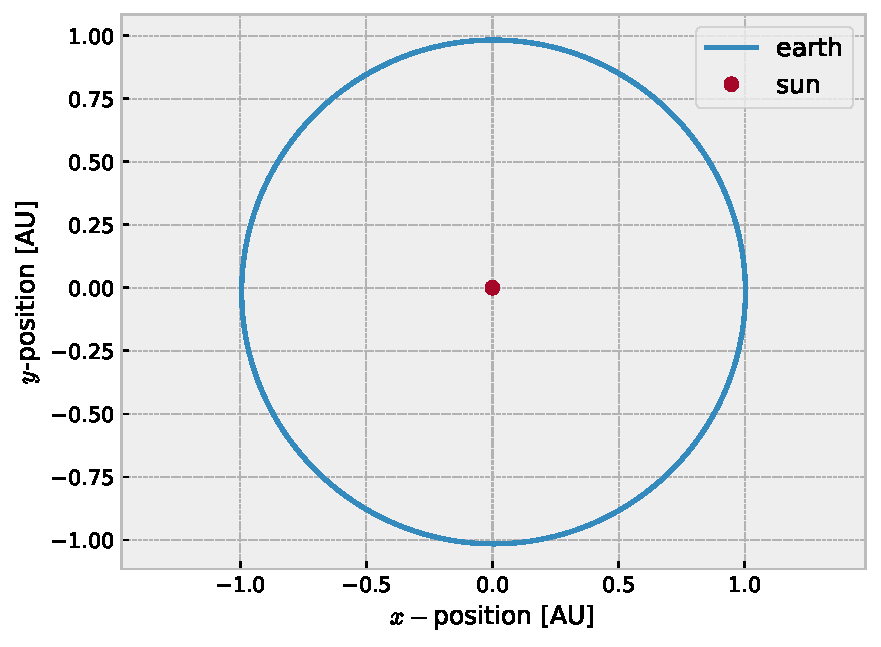
\includegraphics[width=0.45\textwidth]{../figures/eart_sun_orbit.pdf}
  \caption{Position of Earth and Sun over $10$ years with Sun at rest, and the Earth with an initial velocity of $2\pi$, for $N=10^{7}$ data points using the velocity Verlet algorithm. We can clearly see that this initial velocity, with the sun at rest, produces a circular orbit.}
  \label{fig:orbit_Sun_Earth}
\end{figure}

We are interested in finding the deviation of position for different number of data points. We therefore plot the deviation in distance from the final position to the initial position over one year, with an initial velocity of $2\pi$. With this initial velocity the Earth will have a perfectly circular orbit, and the initial and finial position should be equal. The deviation we find between finial and initial position gives us information about the precision of the two algorithms. The deviation in position after one year for different number of data points is shown in figure \vref{fig:deviation_vs_n}.

\begin{figure}
  \centering
  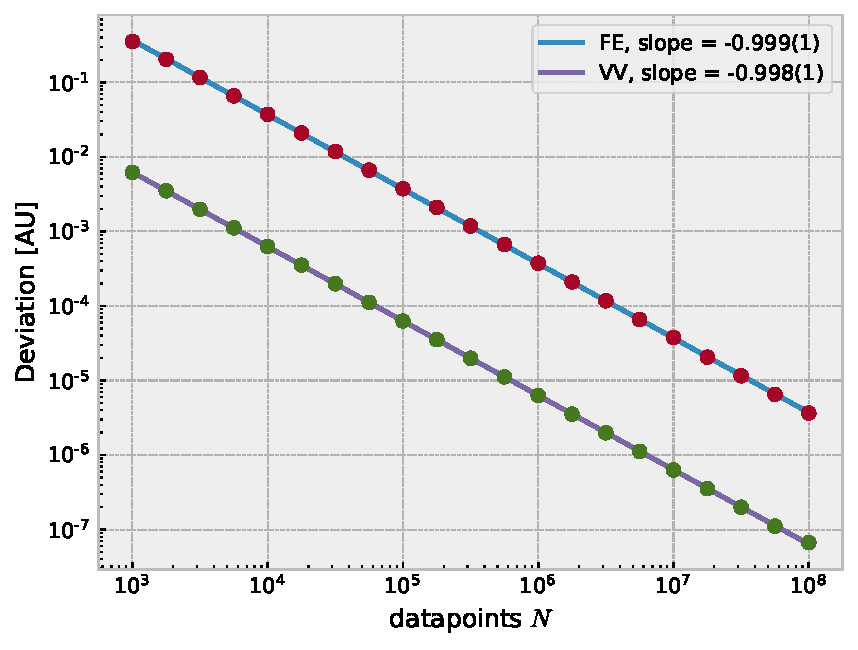
\includegraphics[width=0.45\textwidth]{../figures/deviation_vs_n.pdf}
  \caption{Distance between initial and final position for one year of Earth's orbit as a function of step size using both velocity Verlet and forward Euler. The slope of each algorithm is given in the legend, with it's uncertainty calculated from the least squares method \cite{Squires}. The deviation in position scales almost perfectly linearly with the number of data points.}
  \label{fig:deviation_vs_n}
\end{figure}

For orbits to be stable the energy has to be conserved. We therefore analyze the absolute relative change from the initial value of both angular momentum and energy for the Earth-Sun system over $50$ years. The time evolution of the relative deviation of angular momentum and energy is shown in figure \vref{fig:deviation_E_L}.

\begin{figure}
  \centering
  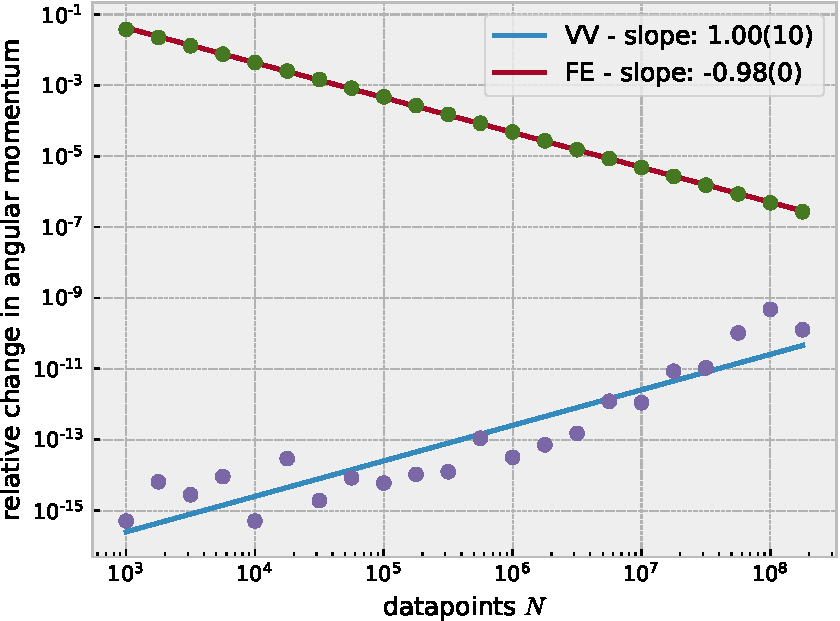
\includegraphics[width=0.45\textwidth]{../figures/deviation_E_L.pdf}
  \caption{Absolute relative difference between initial and later value for total angular momentum and total energy of the system for velocity Verlet and forward Euler. In the legend $E$ is energy and $L$ is angular momentum, where the induces $_{vv}$ and $_{fe}$ refers respectively to the velocity Verlet and forward Euler algorithm. We see that velocity Verlet conserves angular momentum and energy to a precision exceeding all practical purposes, while FE does not. This was calculated with $N=10^{8}$ data points.}
  \label{fig:deviation_E_L}
\end{figure}

In figure \vref{fig:time_relation} the time used by the velocity Verlet and the forward Euler algorithm is shown for different number of data points. As we see from the figure the computational time of velocity Verlet and forward Euler algorithm scales linearly with the number of data points. Using the same data we find that velocity Verlet runs a factor of $0.56(2)$ times slower than forward Euler. If $N$ is number of time steps and $k$ is number of celestial objects in our algorithm, the number of FLOPS for forward Euler is $N\left(5k^2+4\right)$, and velocity Verlet is $2N\left(5k^2 +5\right)$. The results found here were calculated for the Sun-Earth system with the sun at rest.

\begin{figure}
  \centering
  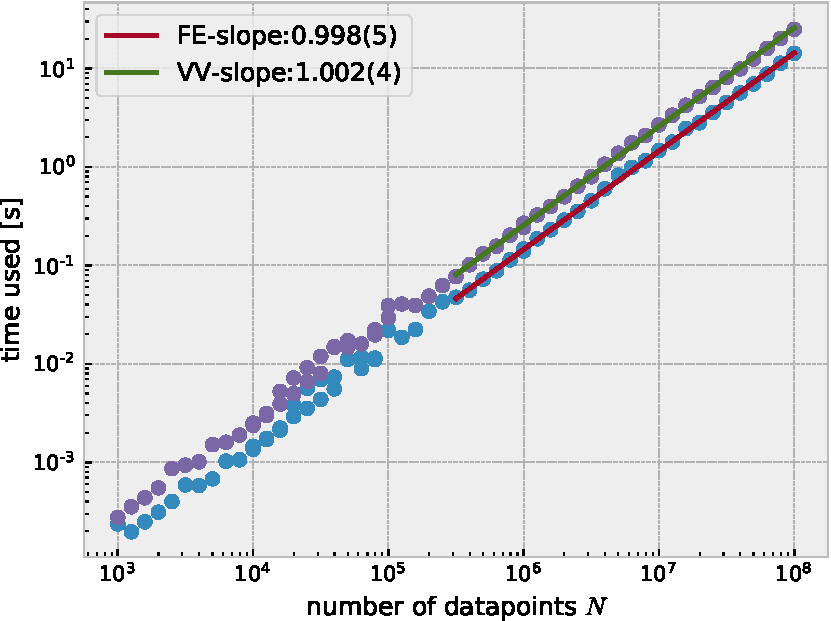
\includegraphics[width=0.45\textwidth]{../figures/timer_VV_and_FE.pdf}
  \caption{Time used by the velocity Verlet and forward Euler algorithm to simulate the Earth-Sun system as a function of number of data points. The slope of each algorithm is given in the legend, with it's uncertainty calculated from the least squares method \cite{Squires}. The time used for small number of data points was not included in the calculation of the slope due their unstable behaviour. The blue dots are the measurements using forward Euler, and the purple dots are the measurements using velocity Verlet. We clearly see the linear relationship between computational time and number of data points.}
  \label{fig:time_relation}
\end{figure}

The radial distance of the Earth to the Sun over $50$ years for different exponents in Newton's gravitational law is shown in figure \vref{fig:different_exp}. The values chosen for the exponent in this figure was chosen to show the transition from a stable to an unstable orbit.

\begin{figure}
  \centering
  \includegraphics[width=0.45\textwidth]{../figures/betta_plot2.pdf}
  \caption{Radial distance between the Sun and the Earth over $50$ years for different values of the exponent in Newton's gravitational law \eqref{newton_betta}. The results were found using velocity Verlet algorithm for $10^7$ data points. The values used for $\beta$ was selected to show the transition from stable to unstable orbit. We see how the orbit becomes more unstable as $\beta$ is approaching $3$, and the orbit finally diverges when $\beta=3$.}
  \label{fig:different_exp}
\end{figure}

We can plot the effective potential originating from the generalized gravitational force in Eq. \eqref{eq: beta_force}. The effective potential is given by Eq. \eqref{eq: effective_potential}. When using units of AU, years and Solar masses, and the fact that the velocity of the Earth is $2\pi$ in a circular orbit, we get that $l^2/M_{Earth} = GM_\odot M_{Earth}$. Plotting the effective potential for different values of $\beta$ then gives Fig. \vref{fig: change_beta}. We see that we have one stable equilibrium at $r = 1$
AU for all $\beta < 3$. For $\beta = 3$, we have no equilibriums at all, while for $\beta > 3$, we get an unstable equilibrium for $r = 1$AU.

\begin{figure*}
\centering
\hspace{-1.5cm}
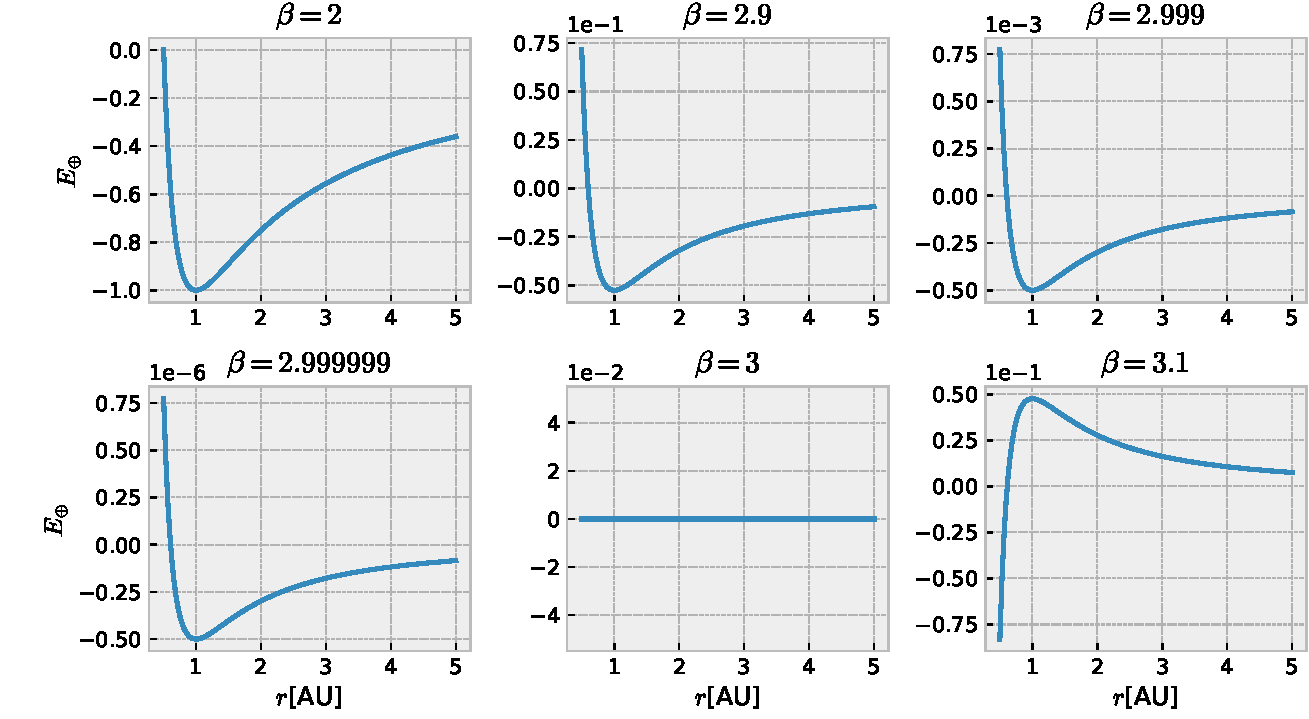
\includegraphics[scale=0.8]{../figures/changing_beta.pdf}
\caption{The effective potential $V_{\mathrm{eff}}$ plotted for different values of $\beta$. The labels on the y-axes are common for all the three plots in a row, while the labels on the x-axes are common for the two plots in the corresponding column. The unit $E_\oplus$ is the absolute value of the energy of the Earth in it's stable orbit for ordinary gravitational force. We see how the scale of the effective potential approaches zero as $\beta\rightarrow 3$, and is exactly equal for $\beta=3$, and has inverted it's shape once $\beta >3$. For $\beta>3$ we have an unstable equilibrium at $1$AU.}
\label{fig: change_beta}
\end{figure*}

We are interested in finding the initial velocity needed for the Earth to escape the gravitational pull of the Sun. The radial distance of the Earth to the Sun is therefore shown as a function of time for different initial velocities in figure \vref{fig:escape_velocity}. In this figure we have chosen to show the last values used in the bisection Method. We find that the initial velocity needed to escape the Sun is $8.8851(5)$AU/year.

\begin{figure}
  \centering
  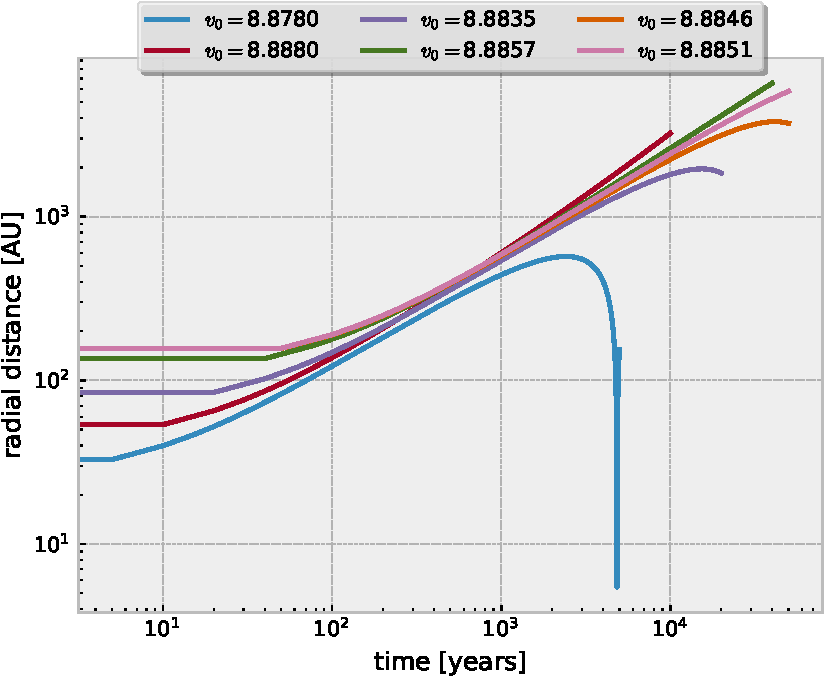
\includegraphics[width=0.45\textwidth]{../figures/escape_velocity.pdf}
  \caption{Radial distance of the Earth as a function of time for different values of the initial velocity, with an initial distance of $1$AU away from the sun. Different velocities were run over different time periods to see if the orbit was closed or not. All runs had the same time step of $2.7$ minutes. The velocities in the legend is given in AU/years. We can tell that the earth needs a velocity of $8.8851(5)$ in order to escape.}
  \label{fig:escape_velocity}
\end{figure}

We want to find the effect that Jupiter has on the orbit of the Earth. To study this effect we find the change radial distance between the Earth and the Sun with and without Jupiter present, over $24$ years. We do the calculation with the mass of Jupiter altered by a factor of $10^{0}$, $10^{1}$ and $10^{2}$, the results are shown in figure \vref{fig:radial_Jupiter}. To understand what is happening when the mass of Jupiter is is even larger, a factor of $1000$ larger, we show the position of the Earth and Jupiter over $12$ years in figure \vref{fig:Earth_becomes_moon}.

\begin{figure}
  \centering
  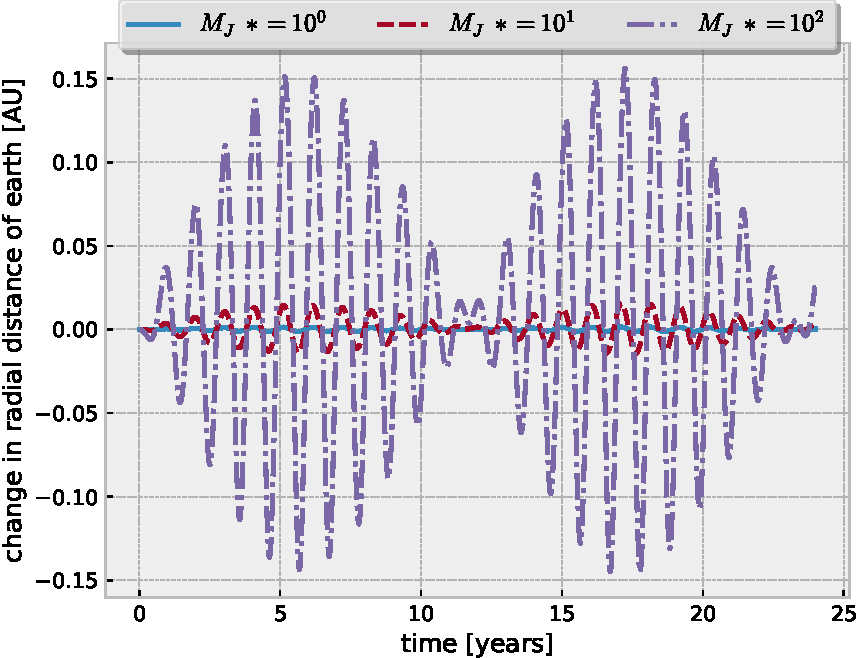
\includegraphics[width=0.45\textwidth]{../figures/radial_distance_jupiter.pdf}
  \caption{The radial distance between the Earth and the Sun is calculated with only these two objects present. We then repeat the calculation including Jupiter in the system. We then calculate the change in position that occurs when Jupiter is included. We do this for three different masses for Jupiter, where it is increased by a factor of $1$, $10$ and $100$. This change in distance is shown over $24$ years. We see that the change in distance is a sum of two sines with very close to equal frequency, resulting in the beating effect we observe here.}
  \label{fig:radial_Jupiter}
\end{figure}

\begin{figure}
  \centering
  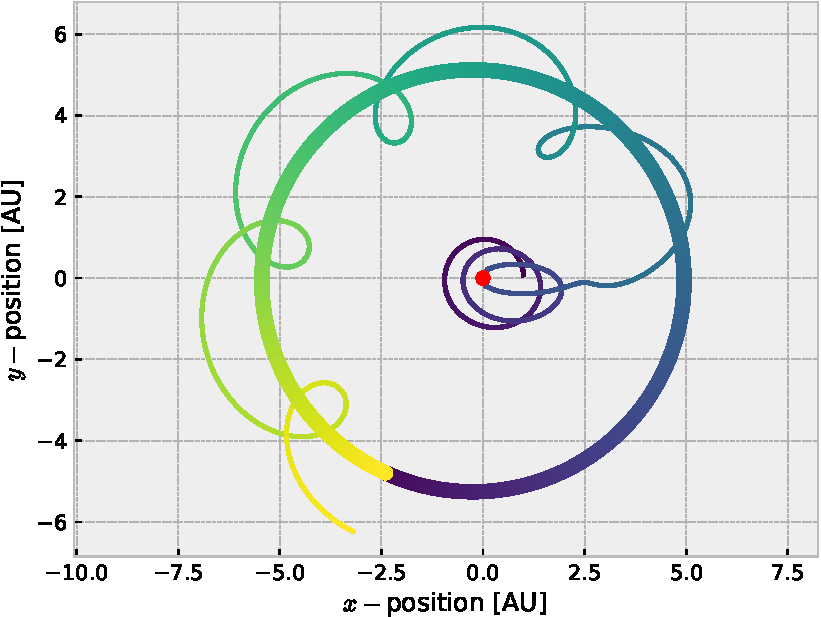
\includegraphics[width=0.45\textwidth]{../figures/jupiter_1000_mass.pdf}
  \caption{The position of the Sun, Earth and Jupiter in the $x-y$ plane over $12$ years with the mass of Jupiter increased by a factor of $1000$. The Sun is the red circle in at the center, the Earth is the thin line, and Jupiter is the thick line. The color of the Earth and Jupiter shows the time evolution of the system, where $t_0$ is dark purple and $t_n$ is light yellow. The same point in time for Earth and Jupiter will have the same colour. We see that the movement of the earth goes from orbiting the Sun to orbiting Jupiter.}
  \label{fig:Earth_becomes_moon}
\end{figure}

In these figures the position of the Sun has been fixed at the origin. The effect of this approximation is shown in figure \vref{fig:effect_of_Sun_at_rest}, where we have plotted the change in position over $24$ years with the Sun at rest compared to not having the Sun at rest.
\begin{figure}
  \centering
  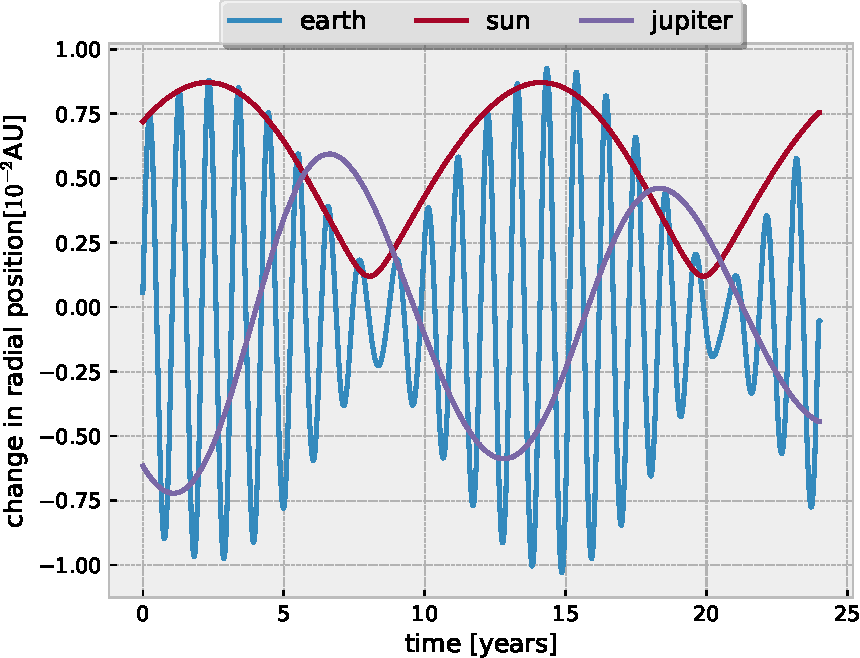
\includegraphics[width=0.45\textwidth]{../figures/sun_movement_effect.pdf}
  \caption{The radial distance to the origin of the Sun, Earth and Jupiter, with the Sun at rest, is subtracted from their respective radial distance without the Sun at rest over. This is shown over a period of $24$ years, and is displayed to see the effect of the approximation of keeping the sun fixed at the origin. The total momentum of the system is set to $0$ at the start of the simulation. System was solved using VV with $10^7$ data points.}
  \label{fig:effect_of_Sun_at_rest}
\end{figure}

In figure \vref{fig:deviation_E_L} we saw the time evolution of energy and angular momentum for the Sun-Earth system. To get a better understanding of the stability of our system we find the relative change in both energy and angular momentum over $12$ years for the Sun-Earth-Jupiter system with VV algorithm as a function of number of data points used. The relative change in energy is shown in figure \vref{fig:conservation_energy}, and the relative change in the angular momentum is shown in figure \vref{fig:change_ang_mom}. These are shown for different masses of Jupiter.

To test the stability as a function of data points we calculate the change in final position of the Earth in the Sun-Earth-Jupiter system as a function of data points, over $12$ years. The result is shown in \vref{fig:change_position}. We do the same for the different masses of Jupiter with the VV algorithm, this is shown in figure \vref{fig:change_position_MJ}.


\begin{figure}
  \centering
  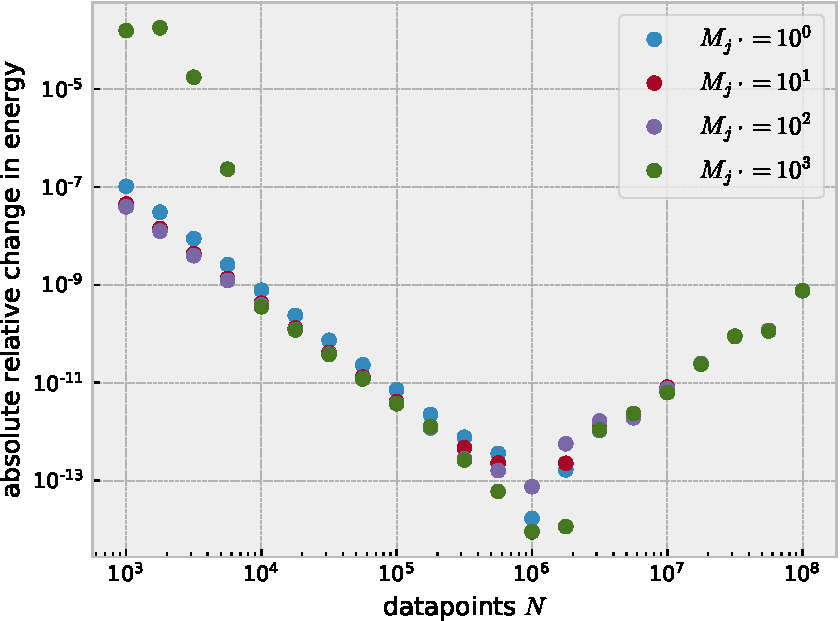
\includegraphics[width=0.45\textwidth]{../figures/conservation_energy2.pdf}
  \caption{The total absolute relative change from initial to final total energy as a function of the number of data points for the Sun-Earth-Jupiter system over $12$ years, for the VV algorithm for different masses of Jupiter. As $N$ increases the deviation get smaller, until a point where the slope changes sign.}
  \label{fig:conservation_energy}
\end{figure}

\begin{figure}
  \centering
  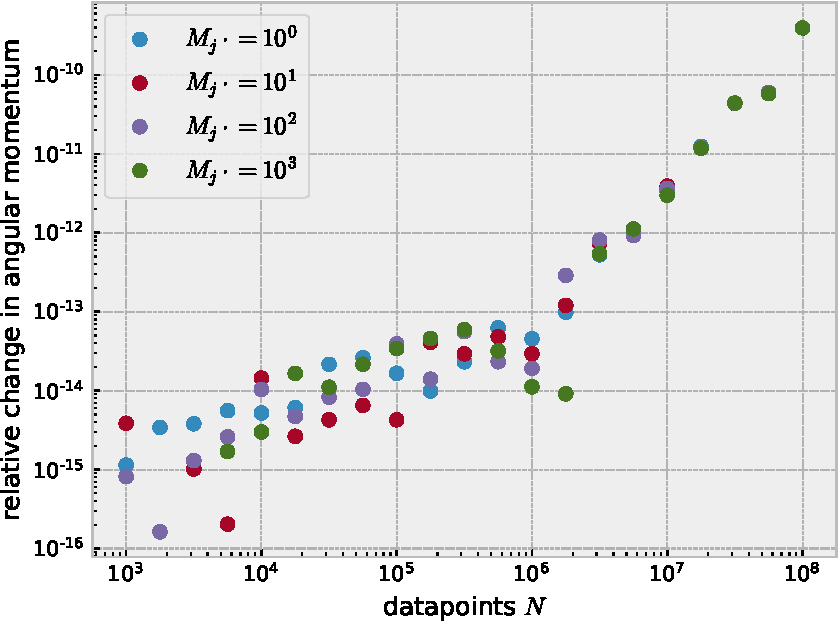
\includegraphics[width=0.45\textwidth]{../figures/conservation_ang_mom_2.pdf}
  \caption{The total absolute relative change from initial to final total angular momentum as a function of the number of data points for the Sun-Earth-Jupiter system over $12$ years, for the VV algorithm for different masses of Jupiter. Contrary to the conservation of energy (shown in figure \vref{fig:conservation_energy}) the conservation of angular momentum gets worse as $N$ increases.}
  \label{fig:change_ang_mom}
\end{figure}

\begin{figure}
  \centering
  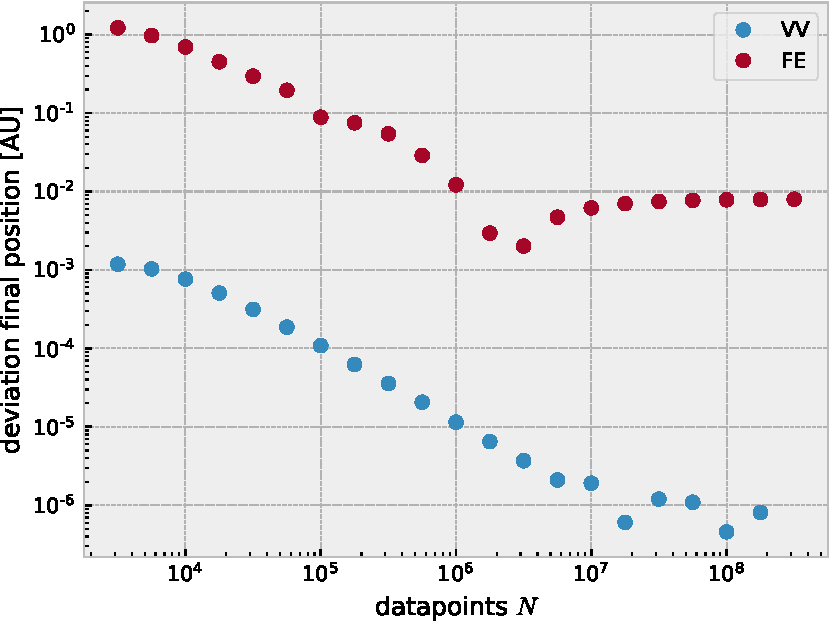
\includegraphics[width=0.45\textwidth]{../figures/change_position.pdf}
  \caption{The absolute change in final position of the earth as a function of the number of data points for the Sun-Earth-Jupiter system over $12$ years, for the VV and FE algorithm. Both algorithms produces a more precise result as the number of data points increases. FE converges to a constant deviation earlier, and for a larger value than VV.}
  \label{fig:change_position}
\end{figure}

\begin{figure}
  \centering
  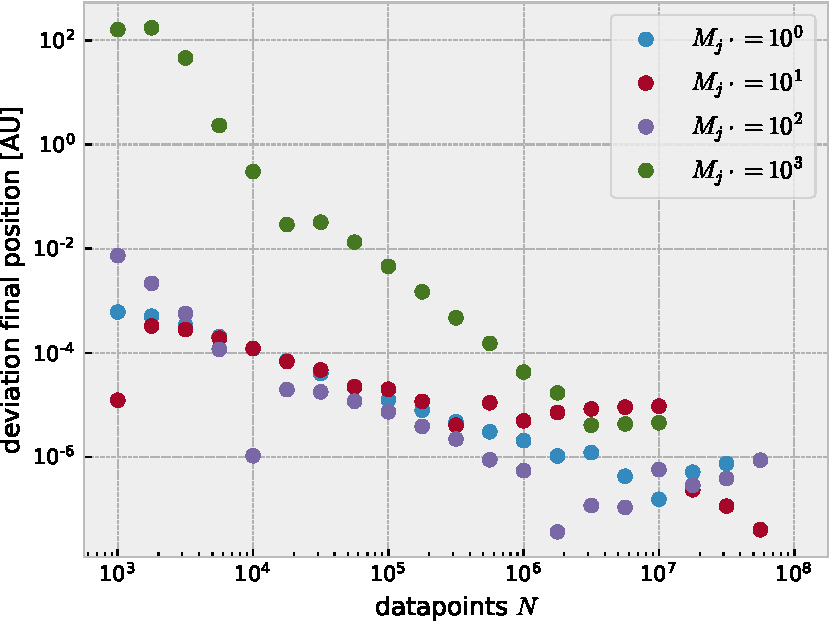
\includegraphics[width=0.45\textwidth]{../figures/change_position_MJ.pdf}
  \caption{The absolute relative change in final position of the earth as a function of the number of data points for the Sun-Earth-Jupiter system over $12$ years, for the VV algorithm for different masses of Jupiter. Both algorithms produces a more precise result as the number of data points increases, up until around $N=10^6$, where the slope goes towards zero.}
  \label{fig:change_position_MJ}
\end{figure}

With our object oriented code it is easy to include additional celestial objects. In figure \vref{fig:total_plot} we show the movement off all the planets, including some moons and Halley's comet over $100$ years.

Simulating the the Sun-Mercury system with the relativistic term to the gravitational force resulted in an observation of the perihelion precision of Mercury. Analytically the perihelion of Mercury will move $42.98^{''}$ per century, and our simulating with $10^{10}$ time steps over $400$ years we found a change in the perihelion of $42.91(1)^{''}$ per century. This is a relative error of $0.17\%$.

\begin{figure*}
  \centering
  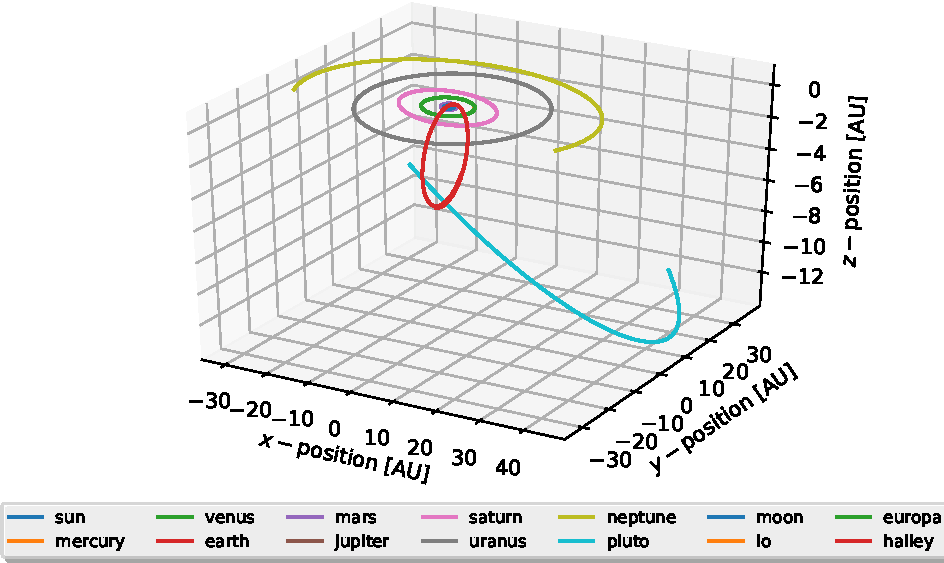
\includegraphics[width=0.9\textwidth]{../figures/total_plot.pdf}
  \caption{Movement of many celestial objects, given in the legend, over $100$ years in three dimensions using velocity Verlet with $10^8$ data points. With this data we will know where all the objects will be in the coming century. The initial position and initial values were collected from NASA.}
  \label{fig:total_plot}
\end{figure*}

\section{Discussion}
\subsection{Velocity Verlet vs forward Euler}
Using natural units makes the initial velocity for a circular orbit $2\pi$ AU/year. We can see this fact in figure \vref{fig:orbit_Sun_Earth} where we achieve a circular orbit with this initial velocity. The movement in that figure was calculated by assuming that the Sun is at rest using the velocity Verlet algorithm. From studying this plot we are not able to find the precision of the algorithm used, since the scale is too large. We therefore analyzed the change in position after one year with an initial condition such that the final and initial position should be the same. This deviation in position as a function of the number of data points is shown in figure \vref{fig:deviation_vs_n}. We see that the both the velocity Verlet and forward Euler has a slope approximately equal to $-1$ in the log-log plot. This means that the total error goes as $N^{-1}$. Forward Euler has a locals error which goes as $N^{-2}$, adding together $N$ of these we will get a total error which goes as $N^{-1}$.
This fits perfectly with the observed error in figure \vref{fig:deviation_vs_n}. Doing the same with velocity Verlet, we find that the total error should go as $N^{-2}$. This is not consistent with what we have measured. This indicates that there is a systematic error present in our calculations or analyzation. Another explanation could be that the final position should not exactly be equal to the initial position, and we are therefore calculating the wrong deviation. If this were the case I would not believe we would find such a small deviation, as well as producing such a linear relationship. A more probable explanation is that the deviation we are finding is not in fact the global error, and we should therefore not expect the slope to be $-2$ for VV. Regardless of the reason, the figure still gives us information about the precision of each algorithm.
\\Even though both algorithms have the same slope, velocity Verlet has a smaller constant term, which makes the final position more precise compared to the position found using forward Euler.\\
Another important quality of an algorithm is how well it conserves angular momentum and energy. For the system we are studying both these properties should be conserved, and we can therefore find which of these two algorithms who are the closes to reproducing this analytical result. In figure \vref{fig:deviation_E_L} the relative deviation of energy and angular momentum is shown as a function of time for $10^{7}$ data points. We see that the velocity Verlet algorithm conserves both the angular momentum and the total energy of the system to a precision exceeding all practical purposes. We see that the change in energy is oscillating over time, with a period of one year. The angular momentum has a more chaotic movement, without any obvious pattern. On the other hand we have Forward Euler, which conserves neither properties accurately. When studying the data without the logarithmic $y$-axis we see that the relative absolute deviation in both angular momentum and energy increases linearly with time, where the energy has a larger slope than the angular momentum. By increasing the number of data points we decrease the change in energy, but for every case the change using velocity Verlet is much smaller. The conservation of energy is one of the most fundamental and important physical laws, and guarantee us that the orbits of the planets are stable over long periods of time. When studying planetary orbits it is therefore vital to have an algorithm which conserves this property. We can therefore be confident in favoring the velocity Verlet algorithm over forward Euler. This is the reason for why we have used velocity Verlet for all the other results.\\
We have seen that the velocity Verlet algorithm produce more precise positions, as well as conserving energy. Are there any downsides to using this algorithm over forward Euler? When counting the number of FLOPS for each algorithm we found that both algorithm scales linearly with the number of time steps, which we can see clearly in figure \vref{fig:time_relation}. Having a linear scaling with number of data points makes the calculation computationally economic, and gives us the possibility of running for very large values of $N$. By calculating the number of FLOPS we find that forward Euler should be approximately, as a function of number of planets, twice as fast as velocity Verlet. This is consistent with the time relationship we measured, which was equal to $0.56(2)$. The exact relationship between the time used by the two algorithms depends on the number of objects included in the algorithm. With more objects the time relationship between the two algorithms should converge two one half. To achieve the values used in figure \vref{fig:time_relation} and a relationship of $0.56(2)$ we studied the Earth-Sun-system.\par
We also studied the stability of the system for the 3-body-problem. In figure \vref{fig:conservation_energy} the relative change in energy is shown as a function of number of data points for different masses of Jupiter using the VV algorithm. We see that VV conserves the total energy more precisely as the number of data points increases, until $N\approx 10^6$, where the slope changes sign, from a value of $-2$ to a value of $2$. By calculating the same graph for FE we get a slope of $-1$, which tells us that VV conserves energy more accurately than FE, which is consistent with what we found in figure \vref{fig:deviation_E_L}. The explanation for the change in slope at $N\approx 10^6$ is due to numerical round off errors. Numerical calculation will result in errors when subtracting two very small numbers, which is occurring in our algorithm. It is therefore not optimal to always increase the number of data points. We see that the conservation of energy is almost identical for different masses of Jupiter, indicating that the complexity of this system does not effect VV's ability to conserve energy, except for small values of $N$ where $M_j\cdot=10^3$ has a larger deviation in energy. We note that we do not observe the round off errors in figure \vref{fig:orbit_Sun_Earth}, where we only have the Earth-Sun system.
This might indicate that the round-off error occurs due to the Earth having two different force sources, which might result in specific values of the acceleration, which will make the calculation of  $\vec{a}_{i+1}+\vec{a}_i$ or $hv_i + h^2\vec{a}_i$ be a subtraction of two small, almost equal values, for certain planet positions.
By comparing the relative change in energy from figure \vref{fig:deviation_E_L} and figure \vref{fig:conservation_energy} we see that VV is able to conserve energy to the same precision for the three body problem, compared to the two body problem. Which is again indicating that the complexity of the system does not effect VV's ability to conserve energy. And that this conservation is more precise than if we were to use FE. \\
Knowing this result we would assume the same when studying the conservation of angular momentum for the same system. Interestingly we observe something completely different, this is shown in figure \vref{fig:change_ang_mom}. Here we see a much more chaotic relationship between conservation accuracy and number of data points, which can locally change in either direction when increasing $N$. This behaviour is also different for different masses of Jupiter. VV still conserves the angular momentum accurately, with a absolute relative deviation down to $10^{-16}$. For the conservation of angular momentum we do observe a change at $N\approx 10^{6}$, but a different change compared to what we observed for the energy (figure \vref{fig:conservation_energy}). For $N > 10^{6}$ VV is able to conserve the angular momentum to the  same precision, regardless of the mass of Jupiter, which it did not do for $N<10^{6}$.
This might indicate that there are different reasons for the observed value in conservation of angular momentum for $N>10^{6}$ and $N<10^{6}$.
For $N>10^{6}$ we believe that the reason for the deviation is numerical round off errors, as we observed for the energy. And that this is the reason for why the different masses of Jupiter is not making a difference in accuracy. For $N<10^{6}$ there must be something different at play, which makes VV conserve angular momentum less precise as $N$ increases, and makes it different for different values of $M_J$. How can it be that VV conserves angular momentum more precisely for large time steps? One could imagine that velocity Verlet is an algorithm constructed to conserve energy, and as a compromise, does not conserve angular momentum accurately. We do not believe this is the reason, as the conservation of angular momentum is closely related to the conservation of energy. Another reason could be that for every time step VV changes the total angular momentum by some constant, and the fewer time steps, the fewer number of iterations changing angular momentum, and the total change is therefore smaller. If this was the case we would observe a more systematic relationship between the conservation and the number of data points, which we do not find here. Perhaps angular momentum is more precisely conserved when the velocity of the planets are constant over longer periods of time, and the path they follow is closer to a polygon than a circle, making fewer time steps more accurate? We do not believe the effect is due to numerical round off errors, as they would be occurring for relatively small values of $N$. Another reason could be a systematic error in our calculations. We do not believe this is likely, since our other results fit well with theory, and our energy behaves as expected, but the chance is there. The most probable solution is that the conservation of angular momentum is not as ordered as the conservation of energy, as we could see in figure \vref{fig:deviation_E_L}, where the change in angular momentum over time seems random. Because of this the change in the total angular momentum is dependent on the time of the measurement, and we can not expect consistent results for different values of $N$. We can still gather information from the data about the approximate conservation of angular momentum when using VV, which we find is very precise. This explanation is consistent with why the error becomes the same for all masses of Jupiter when $N>10^{6}$, since the round off error is the dominating factor in the deviation of angular momentum, where we have a positive slope of $2$, just like we did for energy.
\\
The change in final position of the Earth for the Sun-Earth-Jupiter system is shown as a function of the number of data points over $12$ years in figure \vref{fig:change_position}. As we see both algorithms produce the final position more accurately as the number of data points increases. For FE the deviations converges to around $10^{-2}$AU after around $N=10^{7}$. This is not an accurate final position, and displays the weakness of FE.
Comparing the results shown in figure \vref{fig:deviation_vs_n} and figure \vref{fig:conservation_energy} we can conclude that the stability of FE deteriorates as we include more celestial objects.
We also notice that for small values of $N$, the change in position is extremely large for FE, with a deviation of over $1$AU. The same is not true for VV which starts with a deviation of $10^{-3}$AU, which is lower then the best value produced by FE. In addition VV does not converge as rapidly to a constant value, but we do observe a less steep slope for $N$ larger than $10^{7}$, with a deviation of around $10^{-6}$AU. This is a factor $10^{4}$ more precisely than VV.\\
In figure \vref{fig:change_position_MJ} we displayed the change in final position of the Earth for different masses of Jupiter using the VV algorithm over $12$ years. By increasing the mass of Jupiter by a factor of $1$, $10$ or $100$ we achieve the same behaviour for $N<10^{6}$, where the deviation is quite similar, and decreasing as $N$ increases. By increasing the mass of Jupiter a factor of $1000$ the final position is very sensitive to changes in the number of data points. For small values the change is larger than $100$AU, which is a completely different position. The deviation decreases rapidly as $N$ increases, and is on the same order of magnitude as the other masses when $N\approx 10^{6}$. Around this value of $N$ we see that the deviation converge to a constant, or starts to slightly increase, depending on the mass of Jupiter. This is likely due to round off errors, as we have discussed for the energy and the angular momentum.\\
The only downside to using velocity Verlet compared to forward Euler is that the computational time for a given number of data points is around a factor of two larger. Which we showed in figure \vref{fig:time_relation}. This is a prize worth paying for more precise results and stable orbit through almost perfect conservation of energy and angular momentum, for the right values of $N$.

\subsection{Finding the escape velocity}
We simulated the Earth $1$AU away from the Sun with different initial velocities. By using the bisection method we test with different initial velocities to find the needed velocity for the Earth to escape from the Sun. Analytically we found this velocity to be $2\pi\sqrt{2}\approx 8.8857$, numerically we found it to be equal to $8.8851(5)$AU/year.\\
We had to define an upper limit for when the Earth had escaped the gravitational force from the sun. The upper time limit we chose for our calculations were $45000$ years. With this value we were able to predict the escape velocity of the earth to an accuracy of $0.0068\%$. The analytical and numerical value being this close indicates that our model works.
\\
A problem when finding the needed escape velocity, was that we needed to simulate for such a long period of time to see if the movement was a closed orbit or not. In addition we needed a small time step at the start of the simulation since the velocity of the Earth is large, and it is essential for the beginning of the simulation to be precise, if we want to find the analytical escape velocity. It would be beneficial to use an adaptive method for the time step. At the start of the simulation the Earth has a large velocity, and we need a good precision to find the correct path. Later in the simulation the velocity of the Earth is close to zero, and we do not need a small time step. Implementing an adaptive method would give us the possibility to have a small time step at the start, and a larger one later. This would make it more computationally economical to simulate the path of the Earth over longer periods of time, while keeping a good precision. This would make it easier to check if paths, which seemed to diverge, would diverge or not.
\subsection{Altering Newton's gravitational law}
In addition to changing the initial velocity of Earth, we also tried to alter Newton's gravitational law, and study the orbit of the Earth. The radial distance of the Earth as a function of time is shown in figure \vref{fig:different_exp}, for different values of the exponent in Newton's gravitational law. In this figure we see that increasing the exponent of Newton's gravitational law from $2.0$ to $2.99$ almost has no effect on the orbit of the Earth. We have small oscillations around the equilibrium distance of $1$AU from the Sun. For $\beta$ close to $3$ a small change in potential results in a large change in position. We see that for the exponent $\beta$ equal to $3$ the radial distance from the Sun and the Earth diverges. The Earth is no longer in a stable orbit. For the different values of $\beta$ between $2.99$ and $3.00$ we see that the orbit oscillates with larger and larger amplitudes, with larger and larger periods. Surprisingly we see that the orbit of the Earth is still closed with an exponent of $\beta=2.9998$. \\
The effective potentials shown in figure \vref{fig: change_beta} explain the results seen in Fig. \vref{fig:different_exp}. The closer $\beta$ is to $3$, the weaker is the potential. It is easier to get oscillations about the stable equilibrium of $r=1$AU when the potential is weaker, in other words; the weaker the potential, the bigger the oscillations. The oscillations are due to numerical inaccuracies, and a small numerical inaccuracy can result in a large change in position when the effective potential is weak.
Figure \vref{fig: change_beta} also shows that for $\beta=3$, the potential is zero. Thus, the effective force i zero, and the Earth will not be in a bounded state. For all $\beta > 3$, the initial position of the Earth is an unstable equilibrium, and the orbit will surely not be stable. We also notice that the potential changes much faster for $r<1$AU, and slower for $r>1$AU for $\beta<3$, we notice this effect in figure \vref{fig:different_exp} as well, where we see that all oscillations are only for $r>1$AU, and not for $r<1$AU.

\subsection{The three body problem - Sun, Earth and Jupiter}
We study the three body problem of the Sun, the Earth and Jupiter. This is a problem with no analytical solution, and numerical methods are the best way to find an answer. In figure \vref{fig:radial_Jupiter} the change in radial distance between the Earth and the Sun due to the existence of Jupiter is shown over $24$ years for three different masses of Jupiter. This way we can study how the force on the Earth from Jupiter is effecting the orbit of the Earth. The presence of Jupiter, where the mass is multiplied by a factor of $1$, does not have a large effect on the path of Earth. We just notice small oscillations with a period of one year. This is explained by the fact that the Earth is close to Jupiter once every year, and it gets pulled away from the sun and towards Jupiter. Increasing the mass of Jupiter by a factor of $10$ increases the amplitude of the oscillations, while the period stays fixed. Since the mass of Jupiter increasing implies a stronger gravitational force acting on the Earth it makes sense that the amplitude increases. It also makes sense that the period stays fixed, since the Earth is still doing one revolution each year. When we increase the mass of Jupiter by a factor of $100$ the same happens again; the amplitude increases, but the period stays fixed.
The path of the Earth when we increase the mass of Jupiter by a factor of $1000$ is shown in figure \vref{fig:Earth_becomes_moon}, where we can see that the Earth is becoming one of Jupiter's moons. When we increase the mass of Jupiter by a factor of $1000$ it has approximately the same mass as the Sun. The force acting on the Earth from Jupiter is now so large that it increases the eccentricity of Earth's orbit around the Sun gradually, until the point where the gravitational force from Jupiter is larger than that of the Sun, and the Earth gets pulled towards Jupiter. The Earth is now orbiting Jupiter, and the number of moons on Jupiter has increased by one.
\par
In the simulation we fixed the position of the Sun at the origin, but this is no longer a good approximation when the mass of Jupiter is increased by a factor of $1000$. With this change in mass, the mass of Jupiter is $0.954M_\odot$, and we can therefore no longer assume that the center of mass in the system is inside the Sun. We still used this assumption to study the effect Jupiter has on the Earth's orbit. We did this since we are interested in finding the effect Jupiter has on Earth's orbit. It is therefore use full to fix the position of the Sun, so that it does not get effected by the increase in Jupiter's mass.\par
When forcing the Sun to stand still we are approximating the center of mass of the system to be equal to the center of mass of the Sun. Since the mass of the Sun is more than a factor of $10^6$ larger than the mass of Earth this is a reasonable assumption. The change in gravitational force from such a small change in position is negligible, and this is a reasonable assumption for most cases. Let's study this assumption more closely for the three body problem.\\
When we simulated the three body problem of the Sun, Earth and Jupiter, with the Sun in motion, we set the center of mass of the system as the origin rather than the center of the Sun. We then give the Sun an initial velocity so that the total momentum of all objects is zero. This makes the center of mass stay fixed, and we will avoid having a drifting solar system. In figure \vref{fig:effect_of_Sun_at_rest} we see the change in position for the Sun, Earth and Jupiter with and without the Sun at rest. As we can see, the the Sun has a small orbit around the origin with a period of around $12$ years. This small orbit changes the gravitational force acting on Earth and Jupiter, which changes the force in a noticeable way. The orbit of Earth looks like the product of two sines, one with a small frequency and the other with a large frequency, and this sum creates the beating-effect we see in the data. Such a beating effect will appear when a signal is the sum of two sines with very close frequencies. The change in the radial distance of Jupiter is also oscillating, with around the same frequency as the Sun's, which is equal to the frequency of Jupiter's revolution. We find that the change in position is less than $0.008$AU. For the Sun-Jupiter system we can calculate that the center of mass is a distance of $0.005$AU away from the center of the sun. This is consistent with the value we have observed. If one needs the position of the planets to an accuracy less than one per cent, the assumption about the center of mass of the system being the center of mass of the Sun is not accurate enough.\\By approximating the Sun as the center of mass of the origin we miss out on small oscillations in the radial distance of the planets, as well as for the Sun itself. This oscillations appear since the position of the Sun is now changing over time, and therefore the gravitational force from the Sun to the Planets is also changing. If it is necessary to have a precision for the positions, with less than one per cent the approximation of the Sun being the center of mass is not good enough.

\subsection{Movement of all bodies}
In figure \vref{fig:total_plot} we see the movement of many celestial objects in our Solar system over the coming century. This result was calculated with velocity Verlet over $100$ years, with $10^{8}$ data points. In this figure we can see that the planets are orbiting the Sun in a stable manner, in a two-dimensional plane. Pluto is the exception, with the orbit tilted on an axis compared to the rest of the planets. We see the same for Halley's comet, which has an orbit almost tangential to the plane of the other planets. We see that the movement of all planets are stable over a time period of $100$ years. This is largely because, as we have discussed, the velocity Verlet algorithms ability to conserve energy precisely.

\subsection{Relativistic correction}
By including the relativistic term in Newton's gravitational law we were able to reproduce the analytical value of Mercury's perihelion precision to great accuracy. The relative error we found was equal to $0.17\%$. To achieve this value we used a time step of $1.26$ seconds, and simulated Mercury's movement over $400$ years. Including more terms in the Taylor approximation would not be able to increase our accuracy, over such a small simulation period. The next term would go as $c^{-4}$, where $c$ is the speed of light, which would make the term very small. Could reducing the time step get us a more accurate result? Since the position of the perihelion point is the point closest to the Sun, it is also the point with the largest velocity. We can calculate that the velocity of Mercury at this point is $12.44$AU/year, or $58.98$km/s. With our time step of $1.26$s, this results in a change in position equal to $74.3$km, or $4.96\times 10^{-7}$AU, over one time step. The total distance Mercury travels during one revolutions is $2.41$AU, which would make the change in position over this one time step equal to $2.061\times 10^{-5}\%$ of the total distance traveled, or $0.053^{''}$. Finding the position of the perihelion point within a maximum uncertainty of $0.053^{''}$ is more than enough to observe the drift in it's position over $400$ years. Therefore reducing the time step even further would not necessarily grant us a better result.

\section{Conclusion}
By solving coupled differential equations, through discretizing the continuous equations and using natural units to scale them, we have been able to reproduce analytical results and solve analytically unsolvable problems for the Solar system. Using the results we are able to quantiavly compare two algorithms, forwarad Euler and velocity Verlet. For the Solar system both energy and angular momentum should be conserved. We find that velocity Verlet conserve both of these quantites a factor of more than $10^{4}$ more accurately, as well as producing more accurate positions, as well as it's accuracy not deteriorating as we add more celestial bodies. The only downside to using velocity Verlet over forward Euler is the number of FLOPS, which is around a factor of two larger, resulting in around twice the computational time. Still velocity Verlet is superior due to it's accuracy.\\
Studying the three body problem of the Sun, the Earth and Jupiter, we test our assumption that the center of mass is fixed at the center of the Sun. We find that this assumption changes the position of planets by around $0.008$AU, and should not be assumed to get precice results. When computing the center of mass of the Sun-Jupiter system, we find the center of mass to be $0.005$AU away from the origin, which is quite consistent with what we observed.\\
Using the bisection method we are able to find the escape velocity of the Earth. Analytically the escape velocity is $2\sqrt{2}\pi\approx 8.8857$AU/year, numerically we find it to be equal to $8.8851(5)$, which results to a relative deviation of $0.0068\%$.\\
We alter Newton's gravitational law and check the stability of the Earth's orbit as the exponent approches $3$. We find that Earth's orbit becomes more and more unstable the larger the exponent becomes. When the exponent is exactly equal to $3$ the orbit of the Earth is unstable, and diverges. This is tested versus analytical results from calssical mechanics, and we find complete accordance.\\
By Taylor approximation we add a relativistic term from Einstein's general theory of relativity to Newton's gravitational law. We find that with this additional tem we are able to reproduce the analytical value of Mercury's perihelion precision of $42.98^{''}$ per centrury, numerically with $42.91(1)^{''}$ per centruy, which is a relative deviation of $0.17\%$.\\
Using object orientation we can easily expand the Solar system to an $N$-body problem. And we compute the path of all planets, and some moons over the coming century.


\section{Comments}
All of the code used is available on our GitHub\footnote{\url{http://www.github.uio.no/cecilgl/FYS4150}, and \url{http://www.github.uio.no/ivarsh/FYS4150}}. Here the \texttt{README.MD} files will describe the structure of our GitHub, and what each program was used for. The code itself will also include notes explaining what it does.

\appendix

\section{Generalization of Newton's gravitational law} \label{eom}


We study the modified gravitational force
\begin{equation}
\vec{F} = G\frac{M_\odot M_{Earth}}{r^\beta}\vec{e}_r,
\end{equation}
where $\vec{r}$ is the position vector of the Earth. The corresponding potential is then
\begin{equation}
V = \frac{1}{\beta - 1}\frac{GM_\odot M_{Earth}}{r^{\beta - 1}} = \frac{1}{\alpha}\frac{GM_\odot M_{Earth}}{r^{\alpha}},
\end{equation}
where $\alpha = \beta -1$.


When studying this problem in two dimension, the Earth has two degrees of freedom, and the system can therefore be described by two generalized coordinates: $r$ and $\theta$, as shown in Fig. \vref{fig: Sun-Earth-fig}. The position vector of the Earth is then
\begin{equation}
\vec{r} = r(\cos\theta, \sin\theta).
\end{equation}

The stability of the orbit of the Earth will vary for different values of $\beta$. The Lagrangian of the system is
\begin{equation}
L = K - V = \frac{1}{2}M_{Earth}\left(\dot{r}^2 + r^2\dot{\theta}^2\right) - \left(-\frac{1}{\alpha}\frac{GM_\odot M_{Earth}}{r^\alpha}\right).
\end{equation}

We see immediately from this Lagrangian that there are two constants of motion. The first follows from the fact that there is no explicit time dependence in the Lagrangian. This implies conservation of the Hamiltonian, which in this case is conservation of total energy:
\begin{equation}
\frac{\partial L}{\partial t} \Rightarrow \frac{dH}{dt}.
\end{equation}

The second constant of motion follows from the fact that the generalized coordinat $\theta$ does not appear explicitly in the Lagrangian. Thus, it follows from Lagrange's equation for $\theta$
\begin{equation}
\frac{d}{dt}\left(\frac{\partial L}{\partial \dot{\theta}}\right) - \frac{\partial L}{\partial \theta} = 0,
\end{equation}
that $\frac{\partial L}{\partial \dot{\theta}}$ is conserved. This is
\begin{equation}
\frac{\partial L}{\partial \dot{\theta}} = M_{Earth}r^2\dot{\theta} \equiv l,
\end{equation}
which we interpret as the angular momentum of the Earth relative to the Sun. This can be used to eliminate the $\theta$ dependence in the e.o.m. for the $r$ coordinate:
\begin{equation}
\dot{\theta} = \frac{l}{M_{Earth}r^2}.
\end{equation}

The e.o.m. for the $r$ coordinate is
\begin{align}
\frac{d}{dt}\left(\frac{\partial L}{\partial \dot{r}}\right) - \frac{\partial L}{\partial r} &= 0\\
M_{Earth}\ddot{r} - \left(M_{Earth}r\dot{\theta}^2 - \frac{GM_\odot M_{Earth}}{r^{\alpha + 1}}\right) &= 0\\
M_{Earth}\ddot{r} - \left(\frac{l^2}{M_{Earth}r^3} - \frac{GM_\odot M_{Earth}}{r^{\alpha + 1}}\right) &= 0.
\end{align}

The same e.o.m. will follow from a one dimensional Lagrangian
\begin{equation}
L = \frac{1}{2}M_{Earth}\dot{r}^2 - \left(\frac{1}{2}\frac{l^2}{M_{Earth}}\frac{1}{r^2} - \frac{1}{\alpha}\frac{GM_\odot M_{Earth}}{r^{\alpha}}\right),
\end{equation}
where we define the effective potential as
\begin{equation}
V_{\mathrm{eff}}(r) = \frac{1}{2}\frac{l^2}{M_{Earth}}\frac{1}{r^2} - \frac{1}{\alpha}\frac{GM_\odot M_{Earth}}{r^{\alpha}} \equiv \frac{1}{2}\frac{k}{r^2} - \frac{1}{\alpha}\frac{c}{r^{\alpha}}.
\end{equation}

To have stable equilibrium, this effective potential should have a minimum. We set the derivative with respect to $r$ equal to zero:
\begin{align}
\frac{dV_{\mathrm{eff}}}{dr} &= 0\\
-\frac{k}{r^3} + \frac{c}{r^{\alpha + 1}} &= 0\\
r^{\alpha - 2} &= \frac{c}{k}.\label{eq: stationary}
\end{align}

For the effective potential to be convex, i.e. to have a minima, we get the condition
\begin{align}
\frac{d^2V_{\mathrm{eff}}}{dr^2} &> 0\\
3\frac{k}{r^4} - (\alpha + 1)\frac{c}{r^{\alpha + 2}} &> 0\\
3\frac{k}{r^4} &> (\alpha + 1)\frac{c}{r^{\alpha + 2}}\\
3 r^{\alpha - 2} &> (\alpha + 1)\frac{c}{k}\\
\beta &< 3 r^{\alpha - 2}\frac{k}{c},
\end{align}
which gives
\begin{equation}
\beta < 3,
\end{equation}
when inserting the value for the stationary point in Eq. \eqref{eq: stationary}. Thus, the Earth will have a stable orbit around the Sun for all $\beta < 3$, but for $\beta \geq 3$, we expect the $r$ coordinate to diverge, as there are no stable equilibria.




\bibliography{citations.bib}{}
\bibliographystyle{plain}


\end{document}
%
% ****** End of file apssamp.tex ******
